\documentclass[tikz, border=0mm]{standalone}
\usetikzlibrary{calc}

\definecolor{pGray}{RGB}{160,160,160}

\begin{document}

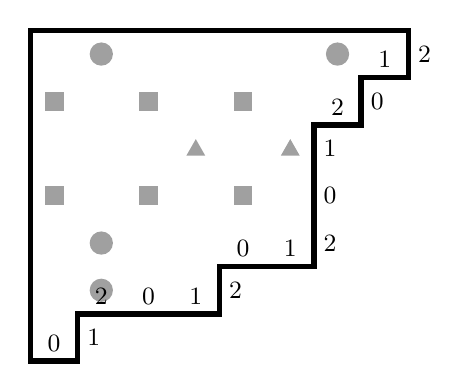
\begin{tikzpicture}[scale=0.6, font=\small]

  % Draw the thick boundary line for partition (8, 7, 6, 6, 6, 4, 1)
  \draw[line width=2pt]
    (0,0) -- (0,7) -- (8,7)
    -- (8,6) -- (7,6) -- (7,5) -- (6,5)
    -- (6,2) -- (4,2) -- (4,1) -- (1,1)
    -- (1,0) -- cycle;

  % Circles
  \foreach \pos in {(1.5, 6.5), (6.5, 6.5), (1.5, 2.5), (1.5, 1.5)} {
    \fill[pGray] \pos circle (7pt);
  }

  % Squares
  \foreach \pos in {(0.5, 5.5), (2.5, 5.5), (4.5, 5.5), (0.5, 3.5), (2.5, 3.5), (4.5, 3.5)} {
    \fill[pGray] \pos +(-0.2,-0.2) rectangle +(0.2,0.2);
  }

  % Triangles
  \foreach \x/\y in {3.5/4.5, 5.5/4.5} {
    \fill[pGray] (\x, \y+0.2) -- (\x-0.2, \y-0.15) -- (\x+0.2, \y-0.15) -- cycle;
  }

  % Boundary Labels
  % Vertical labels on the right side of the drop
  \node[right] at (8, 6.5) {2};
  \node[right] at (7, 5.5) {0};
  \node[right] at (6, 4.5) {1};
  \node[right] at (6, 3.5) {0};
  \node[right] at (6, 2.5) {2};
  \node[right] at (4, 1.5) {2};
  \node[right] at (1, 0.5) {1};

  % Horizontal labels on top of the step
  \node[above] at (7.5, 6) {1};
  \node[above] at (6.5, 5) {2};
  \node[above] at (5.5, 2) {1};
  \node[above] at (4.5, 2) {0};
  \node[above] at (3.5, 1) {1};
  \node[above] at (2.5, 1) {0};
  \node[above] at (1.5, 1) {2};
  \node[above] at (0.5, 0) {0};

\end{tikzpicture}




\end{document}
